%~ \subsection{Model and Implementation}
%~ I will desribe the model in this section in a bottom-up fashion.
%~ First describing all parts and then connecting them.

%~ \subsubsection{Graphs}
    %~ A graph is a set of nodes \(V\) and edges \(E\).
\subsection{Gabriel- and Relative Neighborhood Graph}
\label{ssec:graphtypes}
    All here mentioned graph types are \emph{proximity graphs}. They are
    connecting nodes which are by some metric near to each other.
    Hence they are suited to generalize problems defined on regular
    lattices with nearest neighbor relationships, like the Ising model
    which will be described in more detail in section
    \ref{ssec:isingmodel}.\\
    The Gabriel Graph \cite{Gabriel1969} is a subgraph of the
    Delaunay Triangulation. Two nodes \(i\) and \(j\) with distance
    \(d_{ij}\) are connected with an edge if a circle with it's
    center on the middlepoint between \(i\) and \(j\) and radius
    \(r = \frac d 2\) contains no other nodes. This area will be
    called \emph{lune} in the following. See also Figure
    \ref{fig:lunes}\subref{sfig:lunes:def}.\\
    The Relative Neighborhood Graph \cite{Toussaint1980} is a
    subgraph of the Gabriel Graph. Two nodes \(i\) and \(j\) with
    distance \(d_{ij}\) are connected if no other node is in the
    \emph{lune}. The lune is defined as the intersection of two
    circles with radius \(r = d\) and centers on \(i\) and \(j\).
    See also Figure \ref{fig:lunes}\subref{sfig:lunes:def}.
    \begin{figure}[htbp]
        \centering
        \subfigure[Definition of the lunes][]{
                \label{sfig:lunes:def}
                \tikzset{
    hatch distance/.store in=\hatchdistance,
    hatch distance=10pt,
    hatch thickness/.store in=\hatchthickness,
    hatch thickness=2pt
}

\makeatletter
\pgfdeclarepatternformonly[\hatchdistance,\hatchthickness]{flexible hatch no}
{\pgfqpoint{0pt}{0pt}}
{\pgfqpoint{\hatchdistance}{\hatchdistance}}
{\pgfpoint{\hatchdistance-1pt}{\hatchdistance-1pt}}%
{
    \pgfsetcolor{\tikz@pattern@color}
    \pgfsetlinewidth{\hatchthickness}
    \pgfpathmoveto{\pgfqpoint{0pt}{0pt}}
    \pgfpathlineto{\pgfqpoint{\hatchdistance}{\hatchdistance}}
    \pgfusepath{stroke}
}
\makeatletter
\pgfdeclarepatternformonly[\hatchdistance,\hatchthickness]{flexible hatch nw}
{\pgfqpoint{0pt}{0pt}}
{\pgfqpoint{\hatchdistance}{\hatchdistance}}
{\pgfpoint{\hatchdistance-1pt}{\hatchdistance-1pt}}%
{
    \pgfsetcolor{\tikz@pattern@color}
    \pgfsetlinewidth{\hatchthickness}
    \pgfpathmoveto{\pgfqpoint{0pt}{\hatchdistance}}
    \pgfpathlineto{\pgfqpoint{\hatchdistance}{0pt}}
    \pgfusepath{stroke}
}

\begin{tikzpicture}
    \clip (-2,2.25) rectangle (2,-1.75);

    \begin{scope}
        \clip (-1, 0.5) circle(2.06155281281);
        %~ \fill[fill=blue!20] (1, 0) circle(2.06155281281);
        %~ \draw[pattern=north west lines] (1, 0) circle(2.06155281281);
        \draw[pattern=flexible hatch no,hatch distance=10pt,hatch thickness=0.7pt] (1, 0) circle(2.06155281281);
    \end{scope}

    %~ \fill[fill=white] (0, 0.25) circle(1.0307764064);
    %~ \draw[pattern=north east lines] (0, 0.25) circle(1.0307764064);
    \draw[pattern=flexible hatch nw,hatch distance=10pt,hatch thickness=0.7pt] (0, 0.25) circle(1.0307764064);
    \draw[thick] (0, 0.25) circle(1.0307764064);

    \draw[thick] (-1, 0.5) circle(2.06155281281);
    \fill (-1, 0.5) circle(0.1);
    \draw[thick] (1, 0) circle(2.06155281281);
    \fill (1, 0) circle(0.1);
    \draw[thick] (1, 0) -- (-1, 0.5);
\end{tikzpicture}

        }
        \subfigure[Relative Neighborhood graph example][]{
                \label{sfig:lunes:rng}
                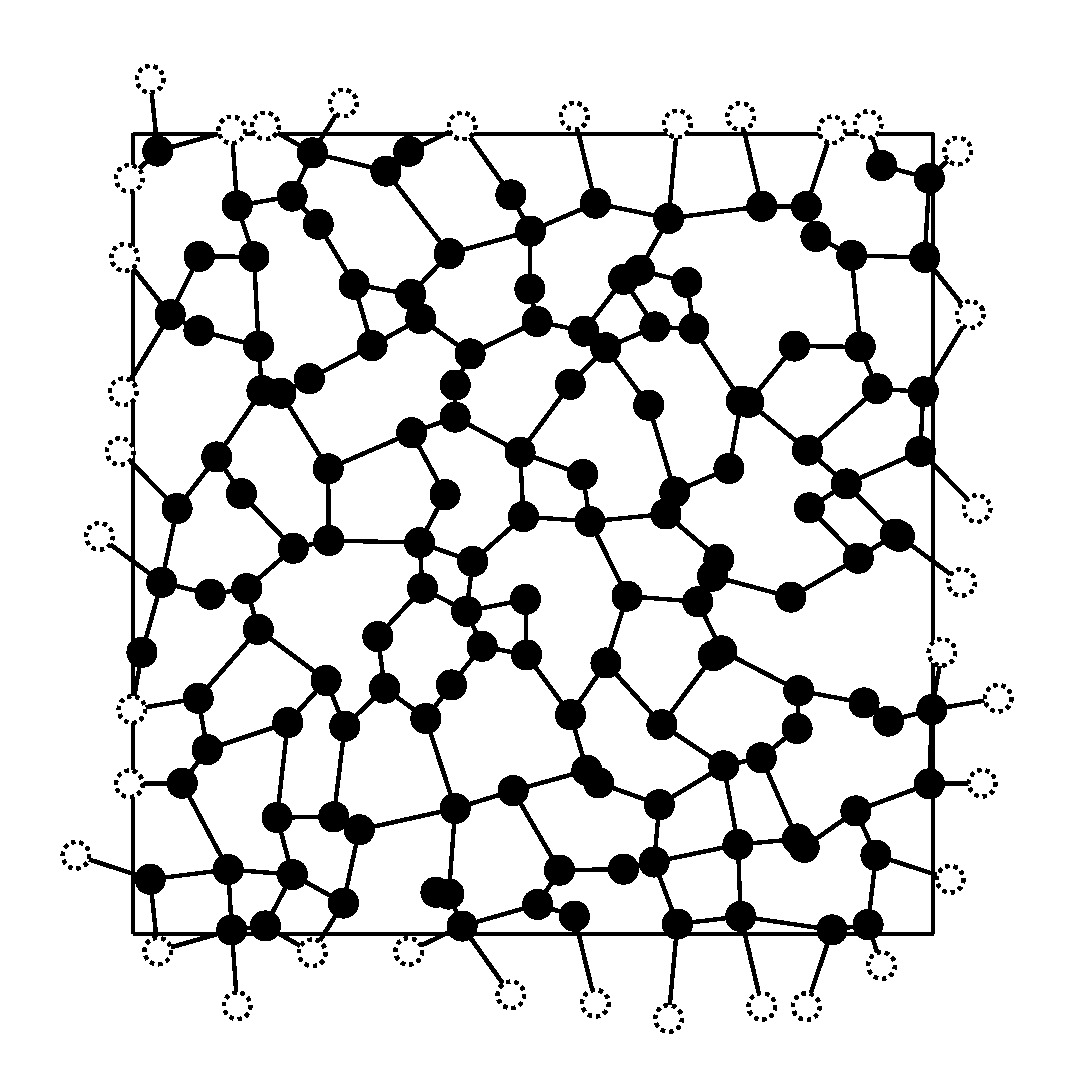
\includegraphics[width=0.3\textwidth]{images/RNG/L12S03.pdf}
        }
        \subfigure[Gabriel graph example][]{
                \label{sfig:lunes:gg}
                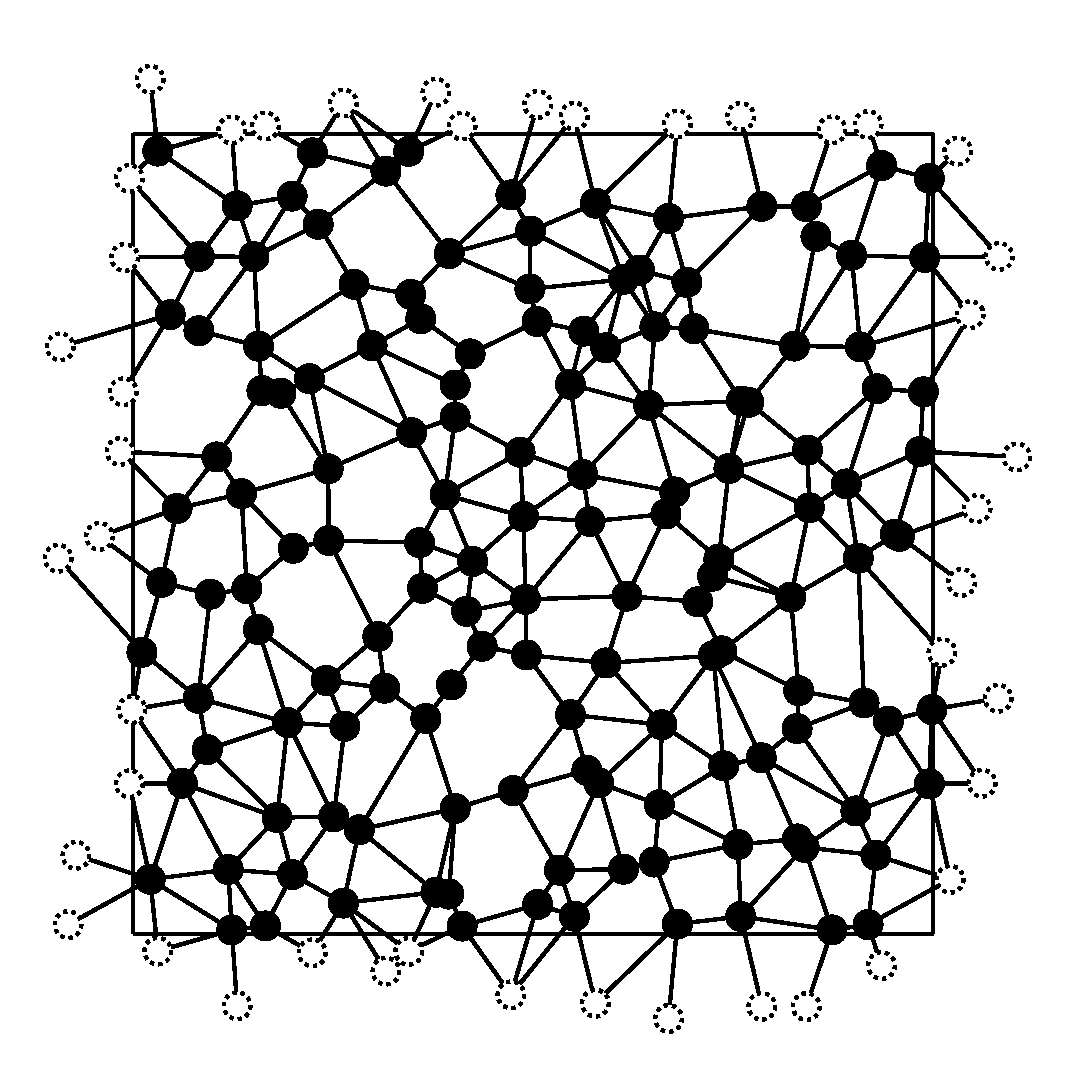
\includegraphics[width=0.3\textwidth]{images/GG/L12S03.pdf}
        }
        \caption[Gabriel - and Relative Neighborhood Graph]
                {\subref{sfig:lunes:def} Lunes of Relative Neighborhood
                    Graph (hatched region) and
                    Gabriel Graph (cross hatched region)
                 \subref{sfig:lunes:def} Example of a Relative
                    Neighborhood Graph on periodic boundary conditions.
                    Periodic nodes are dashed.
                 \subref{sfig:lunes:gg} Example of a Gabriel Graph on
                    periodic boundary conditions. Periodic nodes are
                    dashed.
                }
        \label{fig:lunes}

    \end{figure}

    To construct these graphs the simple way is to test for every
    pair of nodes for every node if it lies in the lune of the pair.
    That is of complexity \(O (n^3)\).\\
    To reduce the complexity one can first create a Delaunay
    Triangulation in complexity \(O (n \log n)\)
    \cite{Leach1992} and test the criterion for each edge, because
    the Delaunay Triangulation is a supergraph of both. But the
    implementation of a Delaunay Triangulation algorithm is not
    trivial and the generation of the graphs is not time critical in
    the scope of this bachelor thesis.\\
    So a tradeoff is to use basicly the simple method but only test
    the criterion for nodes which are near to the lune and abort if
    one node inside the lune is found. To determine which nodes are
    near the lune one can subdivide the area in \emph{cells} and save
    for each cell a list with nodes lying inside it \cite{RNGCell}.
    Now it is just neccessary to test the nodes in the cells which
    resemble a rectangular bounding box of the lune. Most pairs will be
    far away from each other and the cells in the middle of the bounding
    box are completely inside the lune so that only one node has to be
    tested to discard an edge between them. Connected nodes are near to
    each other so that only very few cells have to be tested.\\
    Indeed this method reduced the time needed to construct a Relative
    Neighborhood graph with \(N=32^2\) and \(N=64^2\) by a factor of
    over \(15\) respectivly \(40\). But no further analysis was made.

\subsection{Model}
\label{ssec:isingmodel}
    The used model is a modified 2D Ising model where the \(N\) sites
    are displaced nodes of a square lattice of edge length \(L\) with
    periodic boundary conditions. The displacement is randomly gauss
    distributed with the standard deviation \(\sigma\). This \(\sigma\)
    is also called \emph{disturbance paramter} in the following.
    The hamiltonian of the Ising model is
    \(\hat{H} = \sum_{\avg{i,j}}J_{ij}s_{i}s_{j}\)
    where \(\avg{i,j}\) refers to nodes connected  by edges.
    The edges are constructed according to the in section
    \ref{ssec:graphtypes} defined rules. So that the lattice resembles a
    proximity graph. Each node \(i\) has a spin \(s_i = \pm 1\). Each
    edge has a weight \(J_{ij} = \exp (\alpha (1-d_{ij}))\) with the
    distance \(d_{ij}\) between the nodes \(i\) and \(j\) and
    \(\alpha = 0.5\). \(J\) is called \emph{coupling constant}.\\
    For \(\sigma = 0\) this is the standard Ising model with \(J = 1\),
    for which exists an analytical solution \cite{Onsager1944}.\\

    For evaluation the Monte Carlo simulation is is run till the system
    is equilibrated after \(t_{eq}\) sweeps. Then the simulation continues
    and the magnetisation per site \(m\) and energy per site \(E\)
    are calculated and saved for every \(2\tau\) sweeps. Where \(\tau\)
    denotes the \emph{autocorrelation time} after which two states of
    the system are not correlated anymore.
    For every observable \(O\) the expected value \(\avg{O}\) is averaged
    over different randomly generated lattices \(\overline{\avg{O}}\). The
    errors are estimated by bootstrapping.

\subsection{Critical Temperature $T_c$ and Critical Exponents}
\label{ssec:finitesize}
    The searched for property -- the critical temperature \(T_c\)
    -- is only defined for infinite systems, hence every computer
    simulation will show some \emph{finte size effects}.
    %[vielleicht Bild von intensiver Größe?]
    Despite of this one can obtain \(T_c\) by finite size scaling
    methods \cite[S. ??]{NewmanBarkema1999} which also yield the critical
    exponents. The critical exponents should not be influenced by the
    disturbance paramter \(\sigma\) [citation needed]. So they will be
    used for consistency cross checking and comparision with the known
    exact values \cite[S. 59]{Pelissetto2002}.\\
    %~ [theorie mit dem Collaps]
    %~ [Erklaerung: was sind beta, gamma, nu]
    To accomplish the collapse in an semi-automatic and reproduceable
    way with an error estimate, the programm
    \texttt{autoscale.py} \cite{autoscale2009} is used.
    %~ [Erklärung autoscale]
    %~ [Am besten hier direkt die ganze Auswertung rein]
    %~ [weiter ausarbeiten] [sagen, dass man für zwei/drei sigma die exponenten reproduziert hat].\\
    \begin{figure}[htbp]
        \centering
        \subfigure[Example of a Binder cumulant to determine the critical temperature][]{
                \label{sfig:binder_fit_s_0}
                \includegraphics[width=0.47\textwidth]{plots/binder_fit_s_0}
        }
        \subfigure[Example of a datacollapse to determine critical exponents][]{
                \label{sfig:collapse_s_0}
                \includegraphics[width=0.47\textwidth]{plots/collapse_s_0}
        }
        \caption[Examples of determining critical temperature and exponents]
                {\subref{sfig:binder_fit_s_0} Binder cumulant interpolated
                    with cubic splines (the errorbars are too small to see)
                 \subref{sfig:collapse_s_0} Collapse of the Binder cumulant
                }
        \label{fig:binder_fit_s_0}
    \end{figure}\\
    Though if one is just interested in the critical Temperature, an
    easier approach is to find the intersections of the Binder cumulants
    \(g = 3-\frac{\avg{m^4}}{2\avg{m^2}^2}\) \cite{Binder1981} of different
    system sizes \(L=\sqrt N\).
    Therefore a cubic spline interpolation is calculated\footnote{created using the \texttt{scipy.interpolate} tools \cite{scipy2001}}
    for the measured points.
    In fig. \ref{fig:binder_fit_s_0} such an interpolation is plotted for
    \(\sigma=0\). The cumulants intersect at \(\approx 2.27 k_{B}\). For
    the sake of simplicity let the Boltzmann constant \(k_{B}=1\) in the
    following.
    To determine \(T_c\) the intersections\footnote{found using the \texttt{scipy.optimize} tools \cite{scipy2001}}
    are averaged and the standard
    error is calculated. In this case one gets \(T_c = 2.2689\pm0.0002\),
    which is in good agreement with the exact solution
    \(T_c = 2.2691...\) \cite{Onsager1944}.\\
    Because \(T_{c}\) is dependend on \(J\) and hence also on the count
    of bounds, the values of \(T_{c}\) will be normalized by the mean
    sum of the coupling constants to all neighbors \(\avg{\sum_{\avg{i,j}} J_{ij}}\).

    % The arithmetic average of the intersections are plotted [hier schon?]
    %~ [Und den rest der Auswertung]

% Erwahnen, dass T_c Graph so aussieht, wie degree graph
% mit theo ergebnissen von Honeycomb \cite{Wannier1945} vergleichen (fur deg = 3)
% cosh(2L_c)=2 mit L_c = J/2kT_c -> T_c \approx 1.52
